\entry{2026-10-22}{Improvement campaign, wave 1}

Coordinator campaign \path{reports/2026-10-21-improvement-campaign/} (lanes \texttt{exp/2026-10-21-imp-*}). Errors are conditional E0 estimates; POD comparisons are developmental and in-sample. Wave 1 used about 8.3 GPU-h.
\begin{itemize}
\item \textbf{E5, faster step: stop rule fires.} Precontracted Galerkin with ETDRK4 evolves 14--24$\times$ faster than LSPG CN-R at $r=384$ and wins 36 of 38 cases, but its worst error is slightly higher (1.82\,\% vs 1.78\,\%). POD + ECSW with the same step is still faster at $r=384$.
\item \textbf{E6, cheaper nonlinear term: both stop rules fire.} Smaller rules either fail the quadrature check or lose accuracy; the best gain is 1.24$\times$.
\item \textbf{E7, multi-mesh cost: kill criterion fires.} A continuous POD built once and resampled matches our worst error at about $0.1\times$ our full cost on every workload; the comparative multi-mesh cost claim is dropped.
\item \textbf{E3, variable coefficient: gate fails.} The fastest tuned FOM (exponential integrator with a constant-coefficient split) is not slower than our box ROM (0.86--0.92$\times$); no ROM trained.
\item \textbf{E8 Phase A (CPU):} the decoded bank fields carry a large wall-concentrated sine tail; a bank+sine hybrid does not reach the steep-front floor bar. Phase B (coverage retrain) is running; E2 (geometry) and E1 (box family width) are running.
\end{itemize}
\begin{center}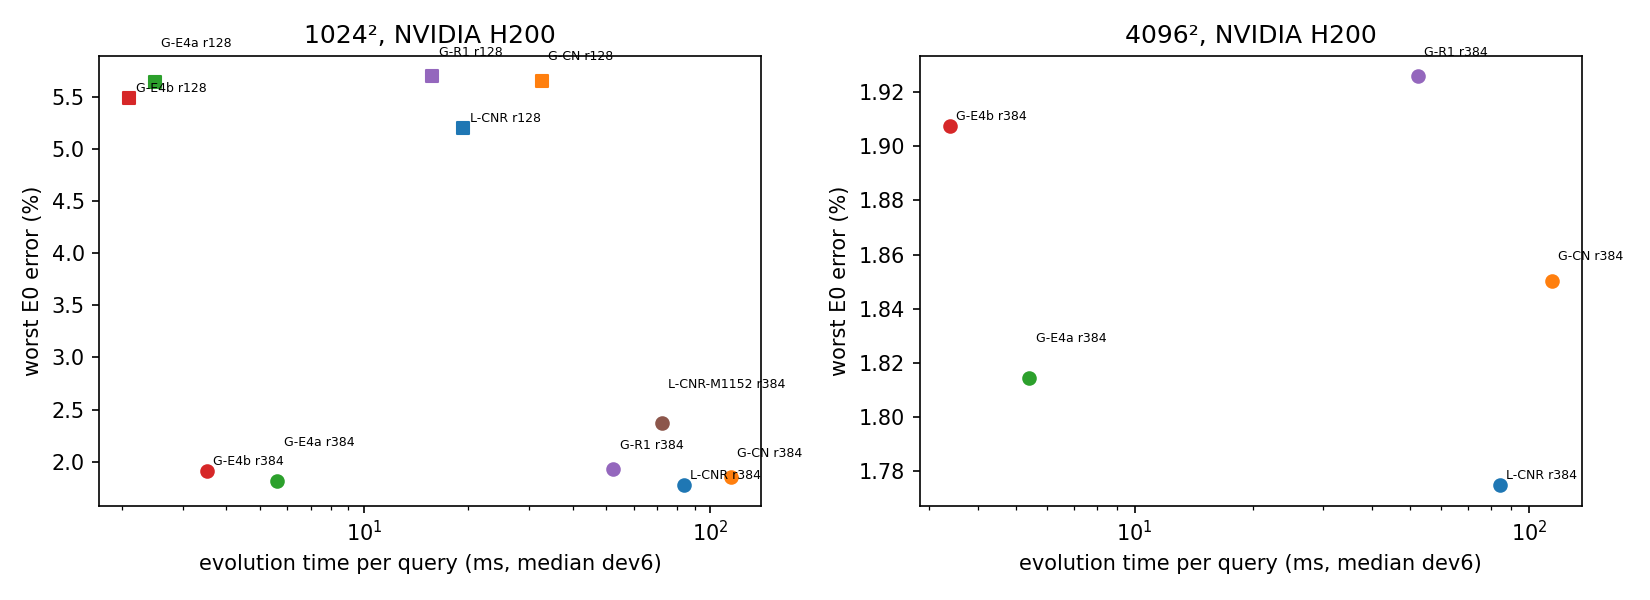
\includegraphics[width=0.48\linewidth]{figs/imp_e5_worst_vs_time.png}\hfill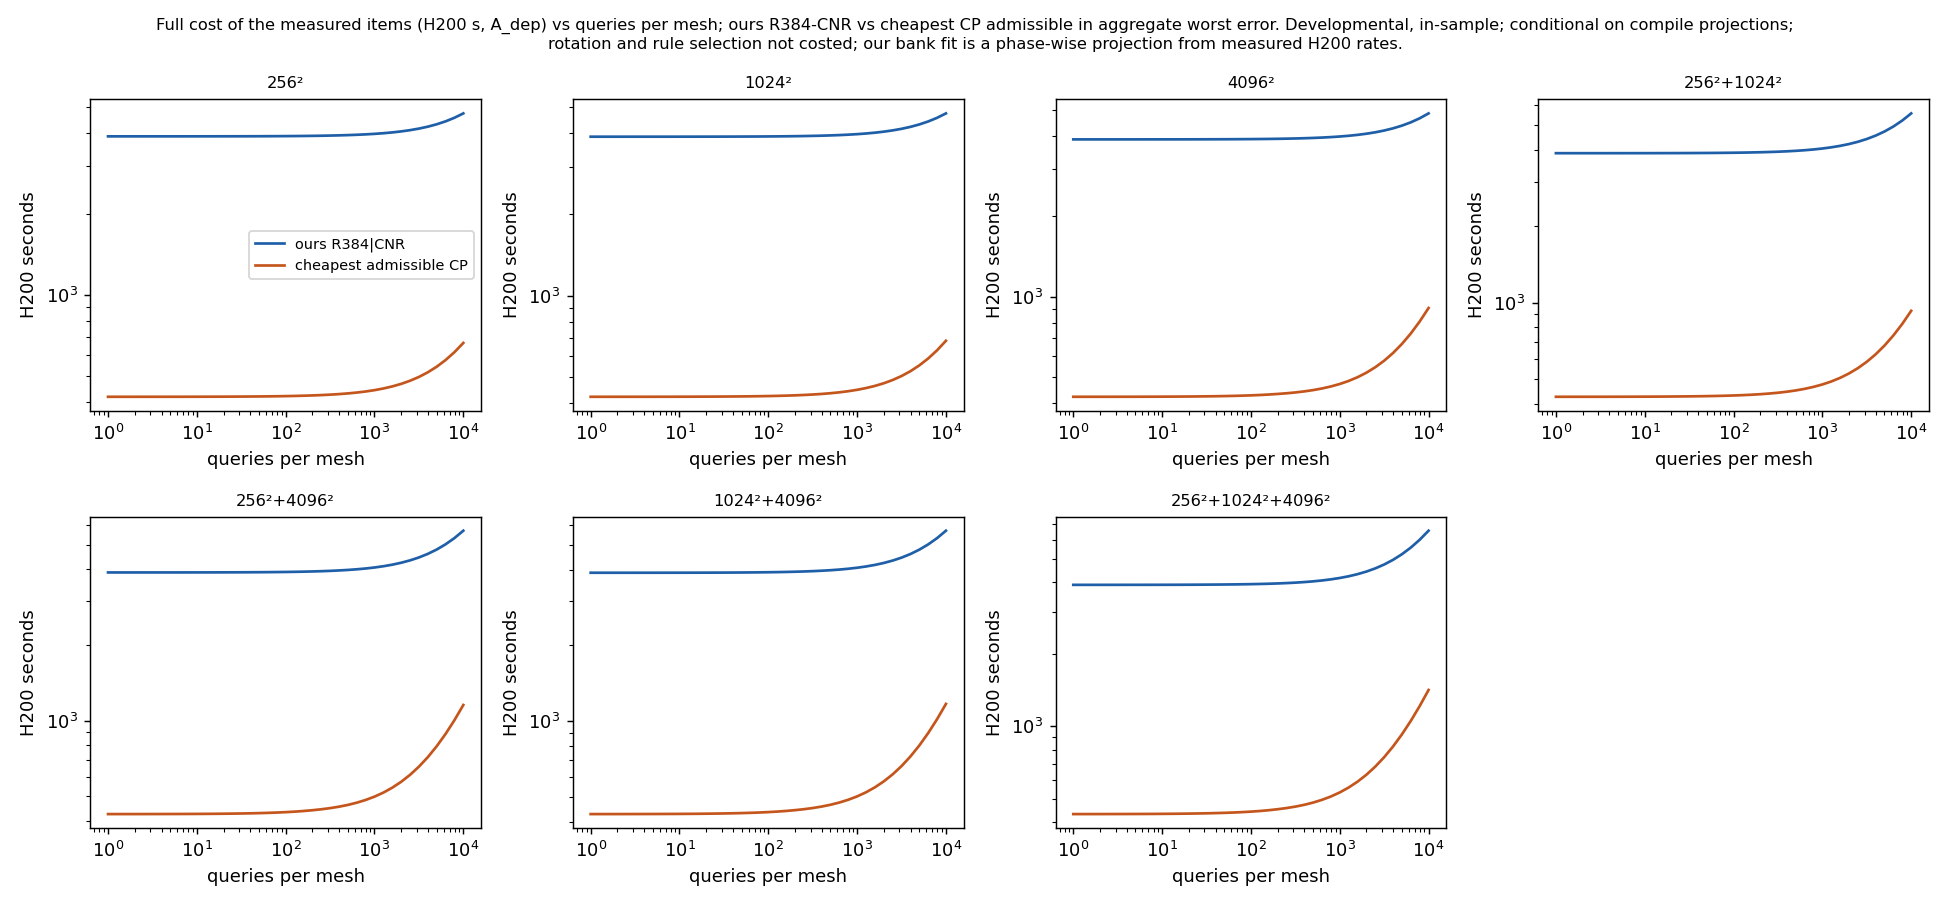
\includegraphics[width=0.48\linewidth]{figs/imp_e7_cost_vs_queries.png}\end{center}
